% mainfile: ../../main.tex
\chapter{Filter-function formalism for unital quantum operations}\label{ch:ff:theory}
We begin the theoretical part of this article by showing how a superoperator matrix representation of the error process, the \enquote{error transfer matrix}, of a unital quantum operation can be computed from the control matrix of the pulse implementing the operation.
The control matrix relates the operators through which noise couples into the system to a set of basis operators in the interaction picture and we detail how it can be calculated in a relatively efficient manner for two different situations.
First, we consider a sequence of gates whose control matrices have been precomputed.
Second, we lay out how the control matrix can be obtained from scratch under the assumption of piecewise constant control, which is often convenient for approximating continuous pulse shapes.
Other wave forms can be dealt with analogously by solving the corresponding integrals.
We then move on to show how several quantities of interest can be extracted and present optimized strategies for computing the central objects of the formalism.

\section{Transfer matrix representation of quantum operations}\label{sec:ff:theory:transfer_matrix}
\subsection{Brief review of quantum operations and superoperators}\label{subsec:ff:theory:quantum_operations}
The quantum operations formalism provides a general framework for the description of open quantum systems~\cite{Kraus1983,Nielsen2011}.
It forms the mathematical basis for \gls{qpt}~\cite{Chuang1997,Poyatos1997} as well as \gls{gst}~\cite{Blume-Kohout2013,Greenbaum2015} and has also been extensively employed in the context of \gls{rb}~\cite{Magesan2011,Kimmel2014}.
Several different representations of quantum operations exist.
While all of them are equivalent one typically chooses the most convenient for the problem at hand.
For an overview of the most commonly used representations see~\citer{Greenbaum2015} and for matrix representations in particular~\citer{Nambu2005} and the references therein.
In this work we employ the Liouville representation, to the best of our knowledge first formalized by~\citet{Fano1957}, to profit from its simple properties under composition.
It is also known as the transfer matrix representation and we will use the terms interchangeably below.
We now briefly review the concept and refer the reader to the literature for further details.
Concretely, the Liouville representation of an operation $\qp: \rho\rightarrow\qp(\rho)$ acting on density operators in a Hilbert space \Hspace of dimension $d$ is given by
\begin{equation}\label{eq:ff:liouville_representation}
\qp_{ij}\doteq\tr(C_i\adjoint\qp(C_j))
\end{equation}
with an operator basis $\basis=\lbrace C_0, C_1, \dotsc, C_{d^2-1}\rbrace$ for the space of linear operators over \Hspace, $\mathsf{L}(\Hspace)$, orthonormal with respect to the Hilbert-Schmidt product $\dotHS{A}{B}\coloneqq\tr(A\adjoint B)$.
In the case that the operator basis corresponds to the Pauli matrices \cref{eq:ff:liouville_representation} is known as the \gls{ptm}.
The operation \qp is thus associated with a $d^2\times d^2$ matrix in \emph{Liouville space} \Lspace that describes its action as the degree to which the $j$ basis element is mapped onto the $i$th.
On \Lspace one can identify a set of basis kets $\lbrace\dket{C_i}\rbrace_{i=0}^{d^2-1} = \lbrace\dket{i}\rbrace_{i=0}^{d^2-1}$ isomorphic to the operators $C_i$ (and correspondingly bras $\dbra{i}$ to the adjoint $C_i\adjoint$) as well as the inner product $\dip{i}{j} = \dotHS{C_i}{C_j}$.
As the vectors $\dket{i}$ form an orthonormal basis, any operator on \Hspace can be written as a vector on \Lspace, $\dket{A} = \sum_i\dket{i}\dip{i}{A}$, whereas a superoperator on \Hspace becomes a matrix on \Lspace, see \cref{eq:ff:liouville_representation}.
It can then be shown that density operators represented by vectors are propagated by transfer matrices so that the action of a quantum operation \qp on a density operator $\rho$ is given by $\dket{\qp(\rho)} = \qp\dket{\rho} = \sum_{ij}\dket{i}\dmel{i}{\qp}{j}\dip{j}{\rho}$.
Thus, the composition of two operations $\qp_1$ and $\qp_2$ corresponds to matrix multiplication in Liouville space, $[\qp_2\circ\qp_1]_{ik} = \sum_j[\qp_2]_{ij}[\qp_1]_{jk}$, a property which makes the representation particularly attractive for sequences of operations.
Although from a numerical perspective the computational complexity scales unfavorably with the system dimension $d$ (\cf \cref{sec:ff:performance:complexity}),  we will employ the Liouville representation for its transparent interpretation and concise behavior under composition in the following analytical considerations.
Lastly, we note that for $C_0\propto\eye$, trace-preservation and unitality are encoded in the relations $\qp_{0j} = \delta_{0j}$ and $\qp_{j0} = \delta_{j0}$, respectively.

\subsection{Liouville representation of the error channel}\label{subsec:ff:theory:transfer_matrix:derivation}
We will now derive an expression for the quantum process of a quantum gate in the presence of arbitrary classical noise.
As a single realization of a classical noise generates strictly unitary dynamics, we will be interested in the expectation value of the dynamics over many such realizations, which will lead to a quantum process including decoherence.
If the noise is additionally Gaussian, these results are exact and therefore apply without restrictions to arbitrarily large noise strength as well as to gates that partially decouple from noise.
For such \glspl{dcg} or \gls{dd} sequences~\cite{Khodjasteh2009,Cywinski2008} higher order terms can become dominant.
In the case that the environment is not strictly Gaussian, our approach becomes perturbative and we recover the results presented in~\citer{Cerfontaine2021}.
As most of our discussion later on in this article will focus on the approximation neglecting coherent errors, readers not interested in the full generality may refer to that publication for a less general but perhaps more accessible derivation and skip ahead to \cref{sec:ff:theory:decay_amplitudes}.

The difference is that in~\citer{Cerfontaine2021}, the Magnus expansion is applied to the solution of the Schrödinger equation, whereas the approach presented here is based on the theory of stochastic Liouville equations and the cumulant expansion~\cite{Kubo1962,Kubo1963}.
In the filter function context, the cumulant expansion has been used to express the decay of the off-diagonal terms of a single-qubit density matrix in~\citer{Cywinski2008}.
More recently,~\citet{Paz-Silva2014} employed it in conjunction with the \gls{me} to obtain the matrix elements of the perturbed density operator after a time $T$ of noisy evolution.
In~\citer{Yang2019a}, the authors made use of the cumulant expansion and stochastic Liouville equations for the purpose of gate optimization.
Here, we combine different aspects of these works and make the connection to the quantum operations formalism by determining the noise-averaged error propagator in the Liouville representation.
This form completely characterizes the error process and hence allows for detailed insight into the decoherence mechanisms of the operation.

Concretely, we consider a system described by the stochastic Hamiltonian
\begin{gather}
    H(t) = \Hc(t) + \Hn(t),\label{eq:ff:hamiltonian} \\
    \Hn(t) = \sum_\alpha b_\alpha(t) B_\alpha(t). \label{eq:ff:hamiltonian:noise}
\end{gather}
$\Hc(t)$ is implemented by the experimentalist to generate the desired control operation during the time $t\in [0, \tau]$ and $\Hn(t)$ describes classical fluctuating noise environments $b_\alpha(t)\in\mathbb{R}$ that couple to the quantum system via the Hermitian noise operators $B_\alpha(t)\in\mathsf{L}(\Hspace)$.
These may carry a general, deterministic time dependence and without loss of generality, we can require them to be traceless since any contributions proportional to the identity do not contribute to noisy evolution in any case.\sidenote{
    The identity commutes with the control Hamiltonian at all times and hence does not generate any evolution in the interaction picture in which we work later on (\cf \cref{eq:ff:cumulant:truncated:substituted})
}
The $b_\alpha(t)$ are random variables drawn from (not necessarily Gaussian) distributions with zero mean that are assumed to be \gls{iid} both with respect to repetitions of the experiment.
Note that this concept of independence does not preclude correlations between different noise sources $\alpha\neq\beta$ nor between one noise source at different times $t\neq t^\prime$, but only serves to obtain a well-defined ensemble average.
Lastly, to be able to later on relate the correlation functions of the $b_\alpha(t)$ to their spectral density, we require the noise fields to be wide-sense stationary, meaning that their correlation function depends only on the time difference.

For noise operators without explicit time dependence, \cref{eq:ff:hamiltonian:noise} constitutes a universal decomposition as can be seen by choosing the $B_\alpha$ from an orthonormal basis for $\mathsf{L}(\Hspace)$.
To motivate the time-dependent form of \cref{eq:ff:hamiltonian:noise}, assume the true Hamiltonian is a function of a set of noisy parameters $\bvec{\tilde{\lambda}}(t) = \bvec{\lambda}(t) + \bvec{\delta\lambda}(t)$ where $\bvec{\delta\lambda}(t) = \text{vec}(\{b_\alpha(t)\}_\alpha)$ are the stochastic variables.
Expanding the Hamiltonian in an orthonormal operator basis yields $H(\bvec{\tilde{\lambda}}(t)) = \sum_\alpha f_\alpha(\bvec{\lambda}(t), \bvec{\delta\lambda}(t)) B_\alpha$.
In general, however, the expansion coefficients $f_\alpha$ will be arbitrary functions of both the deterministic parameters $\bvec{\lambda}(t)$ and the stochastic noises $\bvec{\delta\lambda}(t)$, which prohibits a factorized form like \cref{eq:ff:hamiltonian:noise}.
We can address this problem by first expanding $H$ around $\bvec{\lambda}(t)$ for small fluctuations $\bvec{\delta\lambda}(t)$.
Then, the Hamiltonian approximately becomes $H(\bvec{\tilde{\lambda}}(t)) \approx H(\bvec{\lambda}(t)) + \bvec{\delta\lambda}(t)\cdot\bvec{\nabla}_{\lambda} H(\bvec{\lambda}(t))$, where we can define the control Hamiltonian as $\Hc(t)\coloneqq H(\bvec{\lambda}(t))$.
Expanding the second term in the operator basis now results in the form~\eqref{eq:ff:hamiltonian:noise} for the noise Hamiltonian as it is linear in $\bvec{\delta\lambda}(t)$ and the deterministic time dependence is contained in $\bvec{\nabla}_{\lambda} H(\bvec{\lambda}(t))$ alone.

This permits us to model complex relations between physical noise sources and the noise operators that capture the coupling to the quantum system, arising for example through control hardware or effective Hamiltonians obtained from \eg Schrieffer-Wolff transformations.
While the linearization is in most cases an approximation, it does not impose significant constraints since the noise is typically weak compared to the control.\sidenote{
    The same argument forms the basis for the perturbative approach for non-Gaussian noise.
}
As an example, we could capture a dependence of the device sensitivity on external controls (see also~\citer{Gungordu2018}).
In a widely used setting electrons confined in solid-state quantum dots are manipulated using the exchange interaction $J$ that depends non-linearly on the potential difference $\eps$ between two dots.
Since the dominant physical noise source affecting this control is charge noise, one could include the effect on $J(\eps)$ to first order with $s_\eps(t)=\pdv*{J(\eps(t))}{\eps(t)}$ so that $\Hn(t) = b_\eps(t) B_\eps(t)  =  b_\eps(t) s_\eps(t) B_\eps$ for some operator $B_\eps$ which represents the exchange coupling.

We proceed in our derivation by noting that the control Hamiltonian $\Hc$ gives rise to the noise-free Liouville--von Neumann equation
\begin{equation}\label{liouville-von-neumann}
\dv{\rho(t)}{t} = -\i\comm{\Hc(t)}{\rho(t)} =  -\i\Lc(t)\rho(t)
\end{equation}
on the Hilbert space \Hspace with the Liouvillian superoperator $\Lc(t)$ representing the control.
Analogous to the Schrödinger equation we may also write this differential equation in terms of time evolution superoperators (superpropagators), $\dv*{\liouvUc(t)}{t} = -\i\Lc(t)\liouvUc(t)$ where the action of \liouvUc on a state $\rho$ is to be understood as $\liouvUc\!: \rho\rightarrow\Uc\rho\Uc\adjoint$ with \Uc the usual time evolution operator satisfying the corresponding Schrödinger equation.
This allows us to write the superpropagator for the total Liouvillian $\Li = \Lc + \Ln$ as $\liouvU(t) = \liouvUc(t)\liouvUe(t)$ where the unitary error superpropagator $\liouvUe(t)$ contains the effect of a specific noise realization in \cref{eq:ff:hamiltonian:noise}.
Next, we transform the noise Liouvillian \Ln to the interaction picture with respect to the control Liouvillian $\Lc$ so that $\liouvUe(t)$ satisfies the modified Liouville equation
\begin{gather}
    \dv{\liouvUe(t)}{t} = -\i\Lnt(t)\liouvUe(t),    \label{eq:ff:le:interaction_picture} \\
    \Lnt(t) = \liouvUc^\dagger(t)\Ln(t)\liouvUc(t). \label{eq:ff:liouvillian:interaction_picture}
\end{gather}
\Cref{eq:ff:le:interaction_picture} may be formally solved using the \acrlong{me}~\cite{Magnus1954} so that at time $t=\tau$
\begin{equation}\label{eq:ff:error_propagator}
\liouvUe(\tau) = \exp(-\i\tau\Li_\mr{eff}(\tau))
\end{equation}
with $\Li_\mr{eff}(\tau) = \sum_{n=1}^\infty\Li_{\mr{eff},n}(\tau)$.
A sufficient criterion for the convergence of the expansion is given by~\citet{Moan1999} as $\int_0^\tau\dd{t}\norm*{\Lnt(t)} < \pi$ where $\norm{\placeholder} = \sqrt{\dotHS{\placeholder}{\placeholder}}$ is the Frobenius (Hilbert-Schmidt) norm.
The first and second terms of the \gls{me} are given by~\cite{Magnus1954,Blanes2009}
\begin{subequations}\label{eq:ff:magnus_expansion}
\begin{align}
    \Li_\mr{eff,1}(\tau) &= \frac{1}{\tau}\int_0^\tau\dd{t}\Lnt(t), \label{eq:ff:magnus_expansion:1}\\
    \Li_\mr{eff,2}(\tau) &= -\frac{\i}{2\tau}\int_0^\tau\dd{t_1}\int_0^{t_1}\dd{t_2}\comm{\Lnt(t_1)}{\Lnt(t_2)}. \label{eq:ff:magnus_expansion:2}
\end{align}
\end{subequations}
The $n$ term of the expansion contains $n$ factors of the noise variables $b_\alpha(t)$ and scales with $n$ factors of the control duration $\tau$, suggesting that higher-order terms can be neglected if their product is small.
In the Bloch sphere picture this corresponds to requiring that the angle by which the Bloch vector is rotated away from its intended trajectory due to the noise be small.
Below, we will use the parameter $\xi$ to denote the magnitude of this deviation.
It is properly defined in \cref{subsec:app:ff:convergence:magnus_expansion} where also bounds for the convergence of the \gls{me} are discussed.
Here, we only state that $\Li_{\mr{eff},n}\sim\xi^n$ (see also~\citer{Green2013}).

We have suggestively written the \gls{me} in terms of an effective Liouvillian $\Li_\mr{eff} = \comm{H_\mr{eff}}{\placeholder}$ to interpret it as the generator of a \emph{time}-averaged evolution of a single noise realization up to time $\tau$.
In order to obtain the \emph{ensemble}-averaged evolution of many realizations of the stochastic Hamiltonian in \cref{eq:ff:hamiltonian:noise}, we apply the cumulant expansion to \liouvUe (see also~\citerr{Beaudoin2015}{Willick2018}),
\begin{equation}\label{eq:ff:cumulant_expansion}
\ev*{\liouvUe(\tau)} = \ev{\exp(-\i\tau\Li_\mr{eff}(\tau))} \eqqcolon \exp\cumulantfun(\tau)
\end{equation}
with $\ev{\placeholder}$ denoting the ensemble average\sidenote{
    The ensemble average represents the expectation value over identical repetitions of an operation in an experiment.
    It can be taken to be a spatial ensemble of many identical systems, \eg an NMR system, or, for ergodic systems, a time ensemble of a single system under stationary noise as would be the case for a single spin measured repeatedly, for instance.
}
and the cumulant function~\cite{Kubo1962}
\begin{align}
    \cumulantfun(\tau) &= \sum_{k=1}^\infty\frac{(-\i\tau)^k}{k!}\ev{\Li_\mr{eff}(\tau)^k}_\mr{c} \\
    &= \sum_{k=1}^\infty\frac{(-\i\tau)^k}{k!}\ev{\left[\sum_{n=1}^\infty \Li_{\mr{eff},n}(\tau)\right]^k}_\mr{c}. \label{eq:ff:cumulant}
\end{align}
The notation $\ev{\placeholder}_\mr{c}$ denotes the cumulant average which prescribes a certain averaging operation.
The first cumulant of a set of random variables $\{X_i(t)\}_i$ is simply the expectation value, $\ev*{X_i(t)}_\mr{c} = \ev*{X_i(t)}$, whereas the second cumulant corresponds to the covariance, $\ev*{X_i(t)X_j(t)}_\mr{c} = \ev*{X_i(t)X_j(t)} - \ev*{X_i(t)}\ev*{X_j(t)}$.
Remarkably, third and higher-order cumulants vanish for Gaussian processes~\cite{Kubo1963,Szankowski2017}, making \cref{eq:ff:cumulant} exact by truncating the sums already at $k = 2$ and $n = 2$.
In this case, the convergence radius of the \gls{me} becomes infinite.
The terms with $k = n = 2$ do not contribute as they involve fourth-order cumulants.
Since furthermore we assume that the noise fields $b_\alpha(t)$ have zero mean, also the terms with $k = n = 1$ vanish and $\ev*{X_i(t)X_j(t)}_\mr{c}  =  \ev*{X_i(t)X_j(t)}$.
We can hence write the cumulant function succinctly as
\begin{equation}
    \cumulantfun(\tau) = - \i\tau\ev{\Li_{\mr{eff},2}(\tau)} - \frac{\tau^2}{2}\ev{\Li_{\mr{eff},1}(\tau)^2}  \label{eq:ff:cumulant:truncated}.
\end{equation}
\Cref{eq:ff:cumulant_expansion,eq:ff:cumulant:truncated} allow us to exactly compute the full quantum process $\ev*{\liouvUe}\!: \rho\rightarrow\ev*{\liouvUe(\rho)}$ for Gaussian noise with arbitrary spectral density and power.
For non-Gaussian noise these expressions are approximate up to $\order{\xi^2}$ and higher order terms include both higher orders of the \gls{me} and the cumulant expansion.
Inspecting \cref{eq:ff:cumulant:truncated}, we observe that the first term is anti-Hermitian as it is a pure Magnus term (remember that the \gls{me} preserves algebraic structure to every order) and thus generates unitary, coherent time evolution.
Conversely, the second term is Hermitian and thus generates decoherence.\sidenote{
    In the Liouville representation, the first term is an antisymmetric matrix that generates a rotation and the second a symmetric matrix that generates a deformation of the generalized, $d^2-1$-dimensional Bloch sphere.
}
The former is more difficult to compute than the latter because the second order of the \gls{me}, \cref{eq:ff:magnus_expansion:2}, contains nested time integrals.
Arguments can be made~\cite{Cerfontaine2021}, however, that for single gates in an experimental context the coherent errors captured by this term can be calibrated out to a large degree~\cite{Cerfontaine2020a,Kimmel2015}.
Moreover, many of the central quantities of interest that can be extracted from the quantum process, among which are gate fidelities and certain measurement probabilities, are functions of only the diagonal elements of \cumulantfun.
By virtue of the antisymmetry of the second order terms, they do not contribute to these quantities to leading order as we show in \cref{sec:ff:theory:derived_quantities}.

While we will also lay out how to compute the second order, our discussion will therefore focus on contributions from the incoherent term below.
As it turns out, this term can be computed using a filter function formalism based on that by~\citet{Green2013}.
To see this, we insert the explicit forms of the \gls{me} given in \cref{eq:ff:magnus_expansion} and the noise Hamiltonian given in \cref{eq:ff:hamiltonian:noise} into \cref{eq:ff:cumulant:truncated}.
Together with $\comm{\mc{L}}{\mc{L}'} = \comm{\comm{H}{H'}}{\placeholder}$ and $\mc{L}\mc{L}' = \comm{H}{\comm{H'}{\placeholder}}$, we find that
\begin{align}
    \cumulantfun(\tau) = -\frac{1}{2}\sum_{\alpha\beta}\Biggl(\int_0^\tau\dd{t_1}\int_0^{t_1}\dd{t_2}
    \expval{b_\alpha(t_1) b_\beta(t_2)} & \comm{\comm{\tilde{B}_\alpha(t_1)}{\tilde{B}_\beta(t_2)}}{\placeholder} \notag\\
    +\int_0^\tau\dd{t_1}\int_0^\tau\dd{t_2}
    \expval{b_\alpha(t_1) b_\beta(t_2)} & \comm{\tilde{B}_\alpha(t_1)}{\comm{\tilde{B}_\beta(t_2)}{\placeholder}}\Biggr), \label{eq:ff:cumulant:truncated:substituted}
\end{align}
where $\Bat(t) = \Uc\adjoint(t)\Ba(t)\Uc(t)$ are the noise operators of \cref{eq:ff:hamiltonian:noise} in the interaction picture.
$\ev{b_\alpha(t_1)b_\beta(t_2)}$ is the cross-correlation function of noise sources $\alpha$ and $\beta$ which we will later relate to the spectral density.
For now, we stay in the time domain and introduce an orthonormal and Hermitian operator basis for the Hilbert space \Hspace to define the Liouville representation,
\begin{equation}\label{eq:ff:basis}
    \basis = \bigl\lbrace C_k\in\mathsf{L}(\Hspace): C_k\adjoint = C_k\:\text{and}\:\tr(C_k C_l) = \delta_{kl}\bigr\rbrace_{k=0}^{d^2-1},
\end{equation}
where we choose $C_0 = d^{-\flatfrac{1}{2}}\eye$ for convenience so that the remaining elements are traceless.
In order to separate the commutators from the time-dependence and hence the integral in \cref{eq:ff:cumulant:truncated:substituted}, we expand the noise operators in this basis so that
\begin{equation}\label{eq:ff:noise_operators:expanded}
\Bat(t) \eqqcolon \sum_k\ctrlmat_{\alpha k}(t) C_k.
\end{equation}
The expansion coefficients $\ctrlmat_{\alpha k}(t)\in\mathbb{R}$ are given by the inner product of a noise operator in the interaction picture on the one hand and a basis element on the other:
\begin{equation}\label{eq:ff:control_matrix}
\ctrlmat_{\alpha k}(t) = \langle\Bat(t), C_k\rangle  = \tr(\Uc\adjoint(t)\Ba(t)\Uc(t)C_k).
\end{equation}
In line with~\citet{Green2013}, we call these coefficients the control matrix (see also~\citerr{Byrd2002}{Clausen2010}).
In the transfer matrix (superoperator) picture we can take up the following interpretation for the control matrix by virtue of the cyclicity of the trace: it describes a mapping of a state, represented by the basis element $C_k$ and subject to the control operation $\liouvUc(t): C_k\rightarrow\Uc(t) C_k\Uc\adjoint(t)$, onto the noise operator $\Ba(t)$.
That is, we can write the $\alpha$ row of the control matrix as $\langle\!\langle{\Bat(t)}\rvert = \dbra{\Ba(t)}\liouvUc(t)$.
In this connection lies the power of the \gls{ff} formalism as will become clear shortly; we can first determine the ideal evolution without noise and subsequently evaluate the error process by linking the unitary control operation to the noise operators.

Having expanded the noise operators in the basis \basis, we can already anticipate that upon substituting them, \cref{eq:ff:cumulant:truncated:substituted} will separate into a time-dependent part involving on one hand the control matrix and cross-correlation functions and on the other a time-independent part involving commutators of basis elements.
This will simplify our calculations in the following.
To see this, we recall the definition of the Liouville representation in \cref{eq:ff:liouville_representation} and apply it to the cumulant function so that $\cumulantfun_{ij} = \tr(C_i\cumulantfun[C_j])$, where the notation $\cumulantfun[C_j]$ means substituting $C_j$ for the placeholder $\placeholder$ in the commutators in \cref{eq:ff:cumulant:truncated:substituted} and we suppressed the time argument for legibility.
Finally, we insert the expanded noise operators given by \cref{eq:ff:noise_operators:expanded} and obtain the Liouville representation of the cumulant function,
\begin{equation}
    \cumulantfun_{ij}(\tau) \eqqcolon -\frac{1}{2}\sum_{\alpha\beta} \sum_{kl}\left(
                                                                                  f_{ijkl}\freqshifts_{\alpha\beta,kl} + g_{ijkl}\decayamps_{\alpha\beta,kl}
    \right). \label{eq:ff:cumulant:truncated:liouville}
\end{equation}
Here, we captured the ordering of the noise operators due to the commutators in \cref{eq:ff:cumulant:truncated:substituted} in the coefficients $f_{ijkl}$ and $g_{ijkl}$.
These are trivial functions of the fourth order trace tensor\sidenote{
    Note the similarity to the relationship of a transfer matrix with the $\chi$--matrix, $\qp_{ij} = \sum_{kl}\chi_{kl} T_{i k j l}$, with $\chi_{kl}$ defined by $\qp(\rho) = \sum_{kl}\chi_{kl} C_k\rho C_l$ or, in terms of the Kraus operators $K_i$ of the quantum operation, $\chi_{kl} = \sum_i \tr(K_i C_k) \mr{tr}(K_i\adjoint C_l)  = \left[\sum_i\dop{K_i}{K_i}\right]_{kl}$~\cite{Greenbaum2015}.
}
\begin{equation}\label{eq:ff:trace_tensor}
T_{ijkl} = \tr(C_i C_j C_k C_l)
\end{equation}
given by
\begin{subequations}
    \begin{align}\label{eq:ff:structure_constants}
    f_{ijkl} &= T_{klji} - T_{lkji} - T_{klij} + T_{lkij}\qand \\
    g_{ijkl} &= T_{klji} - T_{kjli} - T_{kilj} + T_{kijl}.
    \end{align}
\end{subequations}
Furthermore, we introduced the frequency (Lamb) shifts \freqshifts and decay amplitudes \decayamps which contain all information on the noise and qubit dynamics as captured by the control matrix $\ctrlmat(t)$:
\begin{align}
    \Delta_{\alpha\beta,kl} &= \int_0^\tau\dd{t_1}\int_0^{t_1}\dd{t_2}\expval{b_\alpha(t_1) b_\beta(t_2)}\ctrlmat_{\alpha k}(t_1)\Rc_{\beta l}(t_2), \label{eq:ff:frequency_shift:time} \\
    \Gamma_{\alpha\beta,kl} &= \int_0^\tau\dd{t_1}\int_0^\tau\dd{t_2}\expval{b_\alpha(t_1) b_\beta(t_2)}\ctrlmat_{\alpha k}(t_1)\Rc_{\beta l}(t_2).  \label{eq:ff:decay_amplitudes:time}
\end{align}
The frequency shifts \freqshifts correspond to the first term in \cref{eq:ff:cumulant:truncated}, hence incurring coherent errors, \ie generalized axis and overrotation errors.
They reflect a perturbative correction to the quantum evolution due to a change of the Hamiltonian at two points in time, and thus time ordering matters.
Conversely, the decay amplitudes \decayamps correspond to the second term and capture the decoherence.
These terms are due to an incoherent average that only takes classical correlations into account, so that time ordering does not play a role.
Note that \cref{eq:ff:cumulant:truncated:liouville} together with \cref{eq:ff:cumulant_expansion} constitutes an exact version (in the Liouville representation) of Eq.~(4) from~\citer{Cerfontaine2021} for Gaussian noise.
The approximation of~\citer{Cerfontaine2021} is obtained by expanding the exponential to linear order and neglecting the second order terms \freqshifts.

For a single qubit and \basis the Pauli basis one can make use of the simple commutation relations so that the cumulant function takes the form (see \cref{sec:app:ff:derivations:cumulant:pauli})
\begin{equation}\label{eq:ff:cumulant:truncated:liouville:pauli}
\cumulantfun_{ij}(\tau) = \begin{cases}
                              - \sum_{k\neq i}\decayamps_{kk}                         &\qif* i = j,   \\
                              - \freqshifts_{ij} + \freqshifts_{ji} + \decayamps_{ij} &\qif* i\neq j,
\end{cases}
\end{equation}
for $i,j > 0$ and any $\alpha,\beta$.
As mentioned in \cref{sec:ff:theory:transfer_matrix} the cases $j = 0$ and $i = 0$ encode trace-preservation and unitality, respectively, and as such $\cumulantfun_{0j} = \cumulantfun_{i0} = 0$ since our model is both trace-preserving and unital.

%Terms on the diagonal of $\cumulantfun(\tau)$ depend only on the diagonal decay amplitudes $\decayamps_{kk}$ and tend to dominate, corresponding to a generalized Pauli channel $\rho\rightarrow\sum_i p_i C_i\rho C_i$ in the weak-noise limit $\ev*{\liouvUe(\tau)}\approx\eye + \cumulantfun(\tau)$. We can intuitively understand this behavior on the basis of the single qubit case by remembering that the transfer matrix of a unitary quantum channel corresponds to a rotation matrix. As each realization of the noise generates a small rotation by $\delta\phi$ about a given axis, expanding the non-trivial elements of the error transfer matrix \liouvUe yields $1 - \flatfrac{\delta\phi^2}{2}$ on the diagonal elements and $\pm\delta\phi$ on the off-diagonals. Subtracting the identity contribution to get the leading-order correction \cumulantfun, we can see that the sign of the off-diagonal terms alternates whereas the diagonal terms are always positive. Therefore, we expect the diagonal terms to typically dominate after taking the ensemble average over many noise realizations.

\section{Calculating the decay amplitudes}\label{sec:ff:theory:decay_amplitudes}
In order to evaluate the cumulant function $\cumulantfun(\tau)$ given by \cref{eq:ff:cumulant:truncated:liouville} and thus the transfer matrix $\ev*{\liouvUe(\tau)}$ from \cref{eq:ff:cumulant_expansion} for a given control operation, we solely require the decay amplitudes $\decayamps_{kl}$ and frequency shifts $\freqshifts_{kl}$ since the trace tensor $T_{ijkl}$ depends only on the choice of basis and is therefore trivial (although quite costly for large dimensions, \cf \cref{sec:ff:performance:basis}) to calculate.
In this section, we describe simple methods for calculating $\decayamps_{kl}$ using an extension of the filter function formalism developed by~\citet{Green2013} that we introduced in~\citer{Cerfontaine2021}.
The central quantity of interest will be the control matrix that we already introduced above.
It relates the interaction picture noise operators to the operator basis and we will compute it in Fourier space in order to identify the cross-correlation functions with the noise spectral density in \cref{eq:ff:decay_amplitudes:time}.
We distinguish between a sequence of quantum gates, as already presented in our related work~\cite{Cerfontaine2021}, and a single gate.
In the first case the control matrix of the entire sequence can be calculated from those of the individual gates, greatly simplifying the calculation if the latter have been precomputed.
This approach gives rise to correlation terms in the expression for $\decayamps_{kl}$ that capture the effects of sequencing gates.
In the second case, as was shown by~\citet{Green2013}, one can calculate the control matrix for arbitrary single pulses under the assumption of piecewise constant control and we lay out how to adapt the approach for numerical applications.

We start by noting that, because we assumed the noise fields $b_\alpha(t)$ to be wide-sense stationary, that is to say the cross-correlation functions evaluated at two different points in time $t_1$ and $t_2$ depend only on their difference $t_1 - t_2$, we can define the two-sided noise power spectral density $S_{\alpha\beta}(\omega)$ as the Fourier transform of the cross-correlation functions $\expval*{b_\alpha(t_1) b_\beta(t_2)}$,
\begin{equation}\label{eq:ff:spectral_density}
\expval{b_\alpha(t_1) b_{\beta}(t_2)} = \int_{-\infty}^{\infty}\ddf{\omega} S_{\alpha\beta}(\omega)\e^{-\i\omega (t_1 - t_2)}.
\end{equation}
Note that the spectrum only characterizes the noise fully in the case of Gaussian noise.
For non-Gaussian components in the noise, additional polyspectra have in principle to be considered for higher-order correlation functions~\cite{Norris2016}.
However, since we only discuss second-order contributions which involve two-point correlation functions here, we only need to take $S_{\alpha\beta}(\omega)$ into account.
Inserting the definition of the spectral density into \cref{eq:ff:decay_amplitudes:time}, one finds
\begin{equation}\label{eq:ff:decay_amplitudes:freq}
\decayamps_{\alpha\beta,kl} = \int_{-\infty}^{\infty}\ddf{\omega}\ctrlmat^\ast_{\alpha k}(\omega)S_{\alpha\beta}(\omega)\ctrlmat_{\beta l}(\omega)
\end{equation}
with $\ctrlmat(\omega) = \int_0^\tau\dd{t}\ctrlmat(t)\e^{\i\omega t}$ the frequency-domain control matrix.
Note that $\ctrlmat^\ast(\omega) = \ctrlmat(-\omega)$ because $\ctrlmat(t)$ is real.
In the above equation, the fourth order tensor
\begin{equation}\label{eq:ff:filter_function:generalized}
\FF_{\alpha\beta,kl}(\omega)\coloneqq\ctrlmat^\ast_{\alpha k}(\omega)\ctrlmat_{\beta l}(\omega)
\end{equation}
is the generalized filter function that captures the susceptibility of the decay amplitudes to noise at frequency $\omega$.
For $\alpha = \beta, k = l$, and by summing over the basis elements,
\begin{equation}\label{eq:ff:filter_function:fidelity}
\FF_{\alpha}(\omega) = \sum_k\bigl\lvert\ctrlmat_{\alpha k}(\omega)\bigr\rvert^2 = \tr(\Bat\adjoint(\omega)\Bat(\omega)),
\end{equation}
and this tensor reduces to the canonical \emph{fidelity} filter function~\cite{Green2012} from which the entanglement fidelity can be obtained, see \cref{subsec:ff:theory:derived_quantities:entanglement_fidelity}.
Thus, if the frequency-domain control matrix $\ctrlmat_{\alpha k}(\omega)$ for noise source $\alpha$ and basis element $k$ is known, the transfer matrix can be evaluated by integrating \cref{eq:ff:decay_amplitudes:freq}.
Moreover, one can study the contributions of each pair of noise sources $(\alpha, \beta)$ both separately or, at virtually no additional cost and to leading order, collectively by summing over them, $\decayamps_{kl} = \sum_{\alpha\beta}\decayamps_{\alpha\beta,kl}$.

We now discuss how to calculate the control matrix $\ctrlmat(\omega)$ in frequency space for a given control operation.
We focus first on sequences of quantum gates, assuming that the control matrices $\ctrlmat\gth{g}(\omega)$ for each gate $g$ have been calculated before.

\subsection{Control matrix of a gate sequence}\label{subsec:ff:theory:control_matrix:sequence}
For a sequence of gates with precomputed interaction picture noise operators the approach developed by~\citet{Green2013} based on piecewise constant control can be adapted to yield an analytical expression for those of the composite gate sequence that is computationally efficient to evaluate~\cite{Cerfontaine2021}.
Here we review these results to give a complete picture of the formalism.
While our results are general and apply to any superoperator representation, we employ the Liouville representation here for its simple composition operation: matrix multiplication.
Computationally, this is not the most efficient choice since transfer matrices have dimension $d^2\times d^2$ and thus their matrix multiplication scales unfavorably compared to, for example, left-right conjugation by unitaries (\cf \cref{sec:ff:performance:complexity}).
However, because the structure of the control matrix \ctrlmat is similar to that of a transfer matrix (remember that it corresponds to a basis expansion of the interaction picture noise operators), we will obtain a particularly concise expression for the sequence in the following.
For a perhaps more intuitive description employing exclusively conjugation by unitaries, we refer the reader to our accompanying publication~\citer{Cerfontaine2021}.

\begin{figure}
    \centering
    \tikzset{slice/.append style={draw=none}}

\begin{quantikz}[align equals at = 1]
	\slice{$t_0$} &
	\gate{P_1} \slice{$t_1$} & 
	\gate{P_2} \slice{$t_2$} & 
	\midstick{$\dotsc$} \slice{$t_{g-1}$} & 
	\gate{P_g} \slice{$t_g$} \arrow[r] &
\end{quantikz}
$=$ 
\begin{quantikz}[align equals at = 1]
	\slice{$t_0$} &
	\gate{Q_g} \slice{$t_g$} \arrow[r] & 
\end{quantikz}

    \caption[Illustration of gate sequence]{
        Illustration of a sequence of $G$ gates.
        Individual gates with propagators $P_g$ start at time $t_{g-1}$ and complete at time $t_g$.
        The total action from $t_0$ to $t_g$ is given by $Q_g$.
    }
    \label{fig:ff:gatesequence}
\end{figure}

A sequence of $G$ gates with propagators $P_g = \Uc(t_g, t_{g-1}), g\in\lbrace 1,\dotsc,G\rbrace$ that act during the $g$ time interval $(t_{g-1}, t_g]$ with $t_0 =  0, t_G = \tau$ as illustrated in \cref{fig:ff:gatesequence} is considered.
The cumulative propagator of the sequence up to time $t_g$ is then given by $Q_g = \prod_{g^\prime=g}^0 P_{g^\prime}$ with $P_0 = \eye$ and its Liouville representation denoted by $\liouvQ\gth{g}$.
Furthermore, the control matrix of the $g$ pulse at the time $t - t_{g-1}$ relative to the start of segment $g$ is
\begin{equation}\label{eq:ff:control_matrix:pulse:time}
\ctrlmat\gth{g}_{\alpha k}(t - t_{g-1}) = \tr(\Uc\adjoint(t, t_{g-1})B_\alpha(t - t_{g-1}) \Uc(t, t_{g-1}) C_k).
\end{equation}
We can now exploit the fact that in the transfer matrix picture quantum operations compose by matrix multiplication to write the total control matrix at time $t\in (t_{g-1}, t_g]$ as
\begin{equation}\label{eq:ff:control_matrix:sequence:time}
\ctrlmat(t) = \ctrlmat\gth{g}(t - t_{g-1})\liouvQ\gth{g-1}.
\end{equation}
The Fourier transform of \cref{eq:ff:control_matrix:sequence:time} can then be obtained by evaluating the transform of each gate separately,
\begin{gather}
    \ctrlmat(\omega) = \sum_{g = 1}^G \e^{\i\omega t_{g-1}}\ctrlmat\gth{g}(\omega)\liouvQ\gth{g-1} \label{eq:ff:control_matrix:sequence:freq}\\
    \ctrlmat\gth{g}(\omega) = \int_0^{\Delta t_g}\dd{t}\e^{\i\omega t}\ctrlmat\gth{g}(t), \label{eq:ff:control_matrix:pulse:freq}
\end{gather}
with $\Delta t_g = t_g - t_{g-1}$ the duration of gate $g$.
Hence, calculating the control matrix of the full sequence requires only the knowledge of the temporal positions, encoded in the phase factors $\e^{\i\omega t_{g-1}}$, and the total intended action $\liouvQ\gth{g-1}$ of the individual pulses if their control matrices have been precomputed.
The sequence structure can thus be exploited to one's benefit.
If the same gates appear multiple times during the sequence one can reuse control matrices for equal pulses to facilitate calculating filter functions for complex sequences with modest computational effort.
Most importantly, \cref{eq:ff:control_matrix:sequence:freq} is independent of the inner structure of the individual pulses and therefore takes the same time to evaluate whether they are highly complex or very simple.
In \cref{sec:ff:performance:complexity}, we will analyze the computational efficiency of capitalizing on this feature in more detail.

As we have seen, the total control matrix of a composite pulse sequence is given by a sum over the individual control matrices.
Since $\ctrlmat(\omega)$ enters \cref{eq:ff:decay_amplitudes:freq} twice, this leads to correlation terms between two gates at different positions in the sequence when computing the total decay amplitudes $\decayamps_{\alpha\beta,kl}$.
Inserting \cref{eq:ff:control_matrix:sequence:freq} into \cref{eq:ff:decay_amplitudes:freq} gives
\begin{align}\label{eq:ff:decay_amplitudes:pulse_correlation}
        \decayamps_{\alpha\beta,kl} &= \begin{aligned}[t]
            \sum_{g,g^\prime=1}^{G}\int_{-\infty}^\infty\ddf{\omega} &
            \bigl[\liouvQ\gthv{g^\prime-1}{\dagger}\ctrlmat\gthv{g^\prime}{\dagger}(\omega)\bigr]_{k\alpha}
            S_{\alpha\beta}(\omega)
            \bigl[\ctrlmat\gth{g}(\omega)\liouvQ\gth{g-1}\bigr]_{\beta l} \\
            &\times\e^{\i\omega(t_{g-1} - t_{g^\prime-1})} \\
        \end{aligned} \notag\\
        &\eqqcolon\sum_{g,g^\prime=1}^{G}\int_{-\infty}^\infty\ddf{\omega} S_{\alpha\beta}(\omega) \FF_{\alpha\beta,kl}\gth{gg^\prime}(\omega)
\end{align}
where we defined the pulse correlation filter function $\FF_{\alpha\beta,kl}\gth{gg^\prime}(\omega)$ that captures the temporal correlations between pulses at different positions $g$ and $g'$ in the sequence.
Unlike regular filter functions, these can be negative for $g\neq g^\prime$ and therefore reduce the overall noise susceptibility of a sequence given by $\FF(\omega) = \sum_{gg^\prime}\FF\gth{gg^\prime}(\omega)$.
We have thus gained a concise description of the noise-cancelling properties of gate sequences: in this picture, they arise purely from the concatenation of different pulses, quantifying, for instance, the effectiveness of \gls{dd} sequences~\cite{Cerfontaine2021}.

\subsection{Control matrix of a single gate}\label{subsec:ff:theory:control_matrix:pulse}
Previous efforts have derived the control matrix analytically for selected pulses such as \gls{dd} sequences~\cite{Cywinski2008}, special dynamically corrected gates (\glspl{dcg})~\cite{Gungordu2018}, as well as developed a general analytic framework~\cite{Green2012,Green2013}.
However, analytical solutions might not always be accessible, \eg for numerically optimized pulses, and are generally laborious to obtain.
Therefore, we now detail a method to obtain the control matrix numerically under the assumption of piecewise constant control.
Our method is similar in spirit to that of~\citet{Green2012} for single qubits with $d=2$, but whereas those authors computed analytical solutions to the relevant integrals during each time step, here we use matrix diagonalization to obtain the propagator of a control operation to make the approach amenable to numerical implementation.
This allows carrying out the Fourier transform of the control matrix \cref{eq:ff:control_matrix} analytically by writing the control propagators in terms of their eigenvalues in diagonal form.

We divide the total duration of the control operation, $\tau$, into $G$ intervals $(t_{g-1}, t_{g}]$ of duration $\Delta t_g$ with $g\in\lbrace 0,\dotsc,G\rbrace$ and $t_0 =  0, t_G = \tau$.
We then approximate the control Hamiltonian as constant within each interval so that within the $g$
\begin{align}\label{eq:ff:hamiltonian:control:piecewise}
\Hc(t) = \Hc\gth{g} = \mr{const.}
\end{align}
and similarly the deterministic time dependence of the noise operators as $\Ba(t) = s_\alpha(t)\Ba = s_\alpha\gth{g}\Ba$.
Under this approximation we can diagonalize the time-independent Hamiltonians $\Hc\gth{g}$ with eigenvalues $\omega_i\gth{g}$ numerically and write the time evolution operator that solves the noise-free Schrödinger equation as $\Uc(t, t_{g-1}) = V\gth{g}D\gth{g}(t, t_{g-1})V\gthv{g}{\dagger}$.
Here, $V\gth{g}$ is the unitary matrix of eigenvectors of $\Hc\gth{g}$ and the diagonal matrix $D_{ij}\gth{g}(t, t_{g-1}) = \delta_{ij}\exp\{-\i\omega_i\gth{g}(t - t_{g-1})\}$ contains the time evolution of the eigenvalues.
Using this result together with $Q_{g-1}$, the cumulative propagator up to time $t_{g-1}$, we can acquire the total time evolution operator at time $t$ from $\Uc(t) = \Uc(t,0) = \Uc(t, t_{g-1}) Q_{g-1}$.
We then substitute this relation into the definition of the control matrix, \cref{eq:ff:control_matrix}, and obtain
\begin{align}
    \ctrlmat_{\alpha k}(t) = s_\alpha\gth{g}&\mr{tr}\Bigl(Q_{g-1}\adjoint V\gth{g} D\gthv{g}{\dagger}(t, t_{g-1}) V\gthv{g}{\dagger} B_\alpha \notag\\
        & \times\,V\gth{g} D\gth{g}(t, t_{g-1})V\gthv{g}{\dagger} Q_{g-1} C_k\Bigr) \\
        \eqqcolon s_\alpha\gth{g}&\sum_{ij}\bar{B}_{\alpha,ij}\gth{g}\bar{C}_{k,ji}\gth{g}
        \e^{\i\Omega_{ij}\gth{g}(t - t_{g-1})}, \label{eq:ff:control_matrix:pulse:time:piecewise}
\end{align}
where $\Omega_{ij}\gth{g} = \omega_i\gth{g} - \omega_j\gth{g}$, $\bar{C}_{k}\gth{g} = V\gthv{g}{\dagger}Q_{g-1} C_k Q_{g-1}\adjoint V\gth{g}$, and $\bar{B}_{\alpha}\gth{g} = V\gthv{g}{\dagger} B_\alpha V\gth{g}$.
Carrying out the Fourier transform of \cref{eq:ff:control_matrix:pulse:time:piecewise} to get the frequency-domain control matrix of the pulse generated by the Hamiltonian from \cref{eq:ff:hamiltonian:control:piecewise} is now straightforward since the integrals involved are over simple exponential functions.
We obtain
\begin{equation}\label{eq:ff:control_matrix:pulse:freq:ff:calculation}
    \ctrlmat_{\alpha k}(\omega) = \sum_{g = 1}^G s_\alpha\gth{g}\e^{\i\omega t_{g-1}}\tr(\bigl[\bar{B}_\alpha\gth{g}\circ I\gth{g}(\omega)\bigr]\bar{C}_k\gth{g})
\end{equation}
with $I_{ij}\gth{g}(\omega) = -\i(\e^{\i(\omega + \Omega_{ij}\gth{g})\Delta t_g} - 1)/(\omega + \Omega_{ij}\gth{g})$ and the Hadamard product $(A\circ B)_{ij}\coloneqq A_{ij}\times B_{ij}$.
\Cref{eq:ff:control_matrix:pulse:freq:ff:calculation} is readily evaluated on a computer and thus enables the calculation of filter functions of arbitrary control sequences, either on its own or in conjunction with \cref{eq:ff:control_matrix:sequence:freq}.
A similar expression is obtained for representations other than the Liouville representation.

\section{Calculating the frequency shifts}\label{sec:ff:theory:frequency_shifts}
The frequency shifts $\freqshifts_{\alpha\beta,kl}$ in \cref{eq:ff:cumulant:truncated:liouville} correspond to the second order of the \gls{me} and thus involve a double integral with a nested time dependence.
This makes their evaluation more involved than that of the decay amplitudes $\decayamps_{\alpha\beta,kl}$ and, in contrast to the previous section, we cannot identify a concatenation rule or single out correlation terms as in \cref{eq:ff:decay_amplitudes:pulse_correlation}.
However, we can still apply the approximation of piecewise constant control and follow a similar approach as in \cref{subsec:ff:theory:control_matrix:pulse} to compute \freqshifts in Fourier space.
Since these terms correspond to a coherent gate error that can in principle be calibrated out in experiments we will not go into much detail here.

We follow the arguments made above for the decay amplitudes and express the cross-correlation functions $\ev{b_\alpha(t) b_\beta(t^\prime)}$ by their Fourier transform, the spectral density $S_{\alpha\beta}(\omega)$, using \cref{eq:ff:spectral_density}.
Inserting this equation into the definition of the frequency shifts in the time domain, \cref{eq:ff:frequency_shift:time}, yields
\begin{equation}\label{eq:ff:frequency_shifts:time}
    \freqshifts_{\alpha\beta,kl} = \int_{-\infty}^\infty\ddf{\omega} S_{\alpha\beta}(\omega)
        \int_0^\tau\dd{t}\ctrlmat_{\alpha k}(t)\e^{-\i\omega t}
        \int_0^t\dd{t^\prime}\ctrlmat_{\beta l}(t^\prime)\e^{\i\omega t^\prime}.
\end{equation}
We again assume piecewise constant time segments so that the inner time integral can be split up into a sum of integrals over complete constant segments $(t_{g^\prime-1},t_{g^\prime}]$ as well as a single integral that contains the last, incomplete segment up to time $t$.
That is, taking the time $t$ of the outer integral to be within the interval $(t_{g-1}, t_g]$ we perform the replacement
\begin{equation}
    \int_0^t\dd{t^\prime} \rightarrow \sum_{g^\prime=1}^{g-1}\int_{t_{g^\prime-1}}^{t_{g^\prime}}\dd{t^\prime} + \int_{t_{g-1}}^{t}\dd{t^\prime}.
\end{equation}
We have thus divided our task into two: The first term allows, as before in \cref{subsec:ff:theory:control_matrix:sequence,subsec:ff:theory:control_matrix:pulse}, to identify the Fourier transform of the control matrix during time steps $g'$ and $g$ for both the inner and the outer integral according to \cref{eq:ff:control_matrix:pulse:freq:ff:calculation}.
The second term remains a nested double integral, but now the integrand contains only products of complex exponentials because we assume the control to be constant within the limits of integration.
As a next step, we also replace the outer time integral by a sum of integrals over single segments, $\int_0^\tau\dd{t}\rightarrow\sum_{g=1}^G\int_{t_{g-1}}^{t_g}\dd{t}$, to obtain
\begin{multline}\label{eq:ff:frequency_shifts:time:substituted}
    \freqshifts_{\alpha\beta,kl} = \int_{-\infty}^\infty\ddf{\omega} S_{\alpha\beta}(\omega)
        \sum_{g=1}^{G}\int_{t_{g-1}}^{t_{g}}\dd{t} \\
        \times\e^{-\i\omega t}\ctrlmat_{\alpha k}(t)
        \left\lbrace\sum_{g^\prime=1}^{g-1}\int_{t_{g^\prime-1}}^{t_{g^\prime}}\dd{t^\prime} + \int_{t_{g-1}}^{t}\dd{t^\prime}\right\rbrace
        \e^{\i\omega t^\prime}\ctrlmat_{\beta l}(t').
\end{multline}
Before continuing, we ease notation and define $\ctrlmat(\omega) \eqqcolon \sum_g\mc{G}\gth{g}(\omega)$ with $\mc{G}\gth{g}(\omega)$ obtained from \cref{eq:ff:control_matrix:pulse:freq:ff:calculation} and furthermore adopt the Einstein summation convention for the remainder of this section, meaning multiple subscript indices that appear on only one side of an equality are summed over implicitly.
We now proceed like in \cref{subsec:ff:theory:control_matrix:pulse} and make use of the piecewise constant approximation to diagonalize the control Hamiltonian during each segment.
For the nested integrals, we obtain $\ctrlmat_{\alpha k}(t)$ from \cref{eq:ff:control_matrix:pulse:time:piecewise}, whereas the remaining integrals factorize and we can identify the Fourier-transformed quantity $\mc{G}\gth{g}(\omega)$.
\Cref{eq:ff:frequency_shifts:time:substituted} then becomes
\begin{multline}\label{eq:ff:frequency_shifts:freq}
    \freqshifts_{\alpha\beta,kl} = \int_{-\infty}^\infty\ddf{\omega} S_{\alpha\beta}(\omega)\sum_{g=1}^G\Biggl[
        \mc{G}_{\alpha k}\gthv{g}{\ast}(\omega)\sum_{g^\prime=1}^{g-1}\mc{G}_{\beta l}\gth{g^\prime}(\omega) \\
        + s_\alpha\gth{g}\bar{B}_{\alpha,ij}\gth{g}\bar{C}_{k,ji}\gth{g} I_{ijmn}\gth{g}(\omega)
        \bar{C}_{l,nm}\gth{g}\bar{B}_{\beta,mn}\gth{g} s_\beta\gth{g}
        \Biggr]
\end{multline}
with $\bar{B}_{\alpha,ij}\gth{g},\bar{C}_{k,ij}\gth{g},\Omega_{ij}\gth{g}$ as defined above in \cref{subsec:ff:theory:control_matrix:pulse} and
\begin{equation}\label{eq:ff:frequency_shifts:integral}
    I_{ijmn}\gth{g}(\omega) = \int_{t_{g-1}}^{t_g}\dd{t}\e^{\i\Omega_{ij}\gth{g}(t - t_{g-1}) - \i\omega t}
        \int_{t_{g-1}}^{t}\dd{t'}\e^{\i\Omega_{mn}\gth{g}(t' - t_{g-1}) + \i\omega t'}.
\end{equation}
Explicit results for the integration in \cref{eq:ff:frequency_shifts:integral} are given in \cref{subsec:app:ff:derivations:frequency_shifts:integral}.
To calculate the frequency shifts \freqshifts, we can thus reuse the quantity $\mc{G}\gth{g}(\omega)$ also required for the decay amplitudes \decayamps.
The only additional computation, apart from contraction, involves the $G$ integrations $I_{ijmn}\gth{g}(\omega)$.
Importantly, \cref{eq:ff:frequency_shifts:freq} has the same structure as the corresponding \cref{eq:ff:decay_amplitudes:freq} for \decayamps in that the individual entries of \freqshifts are given by an integral over the spectral density of the noise multiplied with a -- in this case second-order -- filter function that describes the susceptibility to noise at frequency $\omega$:
\begin{equation}\label{eq:ff:frequency_shifts:filter_function}
    \freqshifts_{\alpha\beta,kl} = \int_{-\infty}^\infty\ddf{\omega} S_{\alpha\beta}(\omega) \FF_{\alpha\beta,kl}\gth{\Delta}(\omega).
\end{equation}

\section{Computing derived quantities}\label{sec:ff:theory:derived_quantities}
By means of \cref{eq:ff:control_matrix:sequence:freq,eq:ff:control_matrix:pulse:freq:ff:calculation,eq:ff:frequency_shifts:freq}, one can obtain the cumulant function $\cumulantfun(\tau)$ from \cref{eq:ff:cumulant:truncated:liouville} and hence the error process $\expval*{\liouvUe(\tau)}$ from \cref{eq:ff:cumulant_expansion} for an arbitrary sequence of gates.
From this, several quantities of interest for the characterization of a given control operation can be extracted.
We explicitly review the average gate and state fidelities as well as expressions to quantify leakage here, but emphasize that this is not exhaustive.
Because for many applications the noise is weak and hence the parameter $\xi\ll 1$, we will in the following expand the exponential in \cref{eq:ff:error_propagator} to leading order in $\xi$ in the following.
That is, we approximate (remember that $\cumulantfun(\tau)\in\order{\xi^2})$
\begin{equation}\label{eq:ff:error_transfer_matrix:approx}
    \ev*{\liouvUe(\tau)}\approx\eye + \cumulantfun(\tau).
\end{equation}
For Gaussian noise, higher order corrections can be obtained either by explicitly calculating higher powers of \cumulantfun or by numerically evaluating the exponential of the cumulant function.
The former method often leads to simpler expressions than \cref{eq:ff:cumulant:truncated:liouville} for which the trace tensor $T_{ijkl}$ need not be computed directly.
In the weak-noise regime, one can also define specific filter functions for each derived quantity that are given in terms of linear combinations of the generalized filter functions $\FF_{\alpha\beta,kl}(\omega)$.
The ensemble expectation value of the quantity can then be obtained directly from the overlap with the spectral density, $\int\flatfrac{\dd{\omega}}{2\pi} \FF(\omega) S(\omega)$.
Finally, we will drop the averaging brackets and the argument of the error transfer matrix $\ev*{\liouvUe(\tau)}$ for brevity in the following.

\subsection{Average gate and entanglement fidelity}\label{subsec:ff:theory:derived_quantities:entanglement_fidelity}
The average gate fidelity is a commonly quoted figure of merit used to characterize physical gate implementations~\cite{Loss1998,Ladd2010,Chow2012,Veldhorst2014,Yoneda2018}.
It represents the fidelity between an implementation \liouvU and the ideal gate \liouvQ averaged over the uniform Haar measure.
Since $\avgfid(\liouvU, \liouvQ) = \avgfid(\liouvQ\adjoint\circ\liouvU, \eye) = \avgfid(\liouvUe)$, the average gate fidelity can be obtained from the error channel \liouvUe as~\cite{Horodecki1999,Nielsen2002}
\begin{align}
    \avgfid(\liouvUe) &= \frac{\tr\liouvUe + d}{d(d+1)} \label{eq:ff:fidelity:avg}\\
    &= \frac{d\times\entfid(\liouvUe) + 1}{d + 1}, \label{eq:ff:fidelity:avg-ent}
\end{align}
where $d$ is the system dimension and $\entfid(\liouvUe) = d^{-2}\tr\liouvUe$ is the entanglement fidelity.
In the low-noise regime where \cref{eq:ff:error_transfer_matrix:approx} holds, we can write the entanglement fidelity in terms of the cumulant function $\cumulantfun_{\alpha\beta}$ approximately as
\begin{align}\label{eq:ff:fidelity:ent}
\entfid(\liouvUe) &= 1 + \frac{1}{d^2}\sum_{\alpha\beta}\tr\cumulantfun_{\alpha\beta} \\
&\eqqcolon 1 - \sum_{\alpha\beta}\infid_{\alpha\beta}(\liouvUe).
\end{align}
Here, we defined $\infid_{\alpha\beta}$, the infidelity due to a pair of noise sources $(\alpha,\beta)$.
As we show in \cref{subsec:app:ff:derivations:fidelity}, we can simplify the trace of the cumulant function so that the infidelity reads
\begin{equation}\label{eq:ff:infidelity:ent}
\infid_{\alpha\beta} = \frac{1}{d}\tr\decayamps_{\alpha\beta}.
\end{equation}
\Cref{eq:ff:infidelity:ent} reduces to Eq.~(32) from~\citer{Green2012} for a single qubit ($d=2$) and pure dephasing noise up to a different normalization convention; by pulling the trace through to the generalized filter function $\FF_{\alpha\beta,kl}(\omega)$ in \cref{eq:ff:decay_amplitudes:freq}, we recover the relation (setting $\alpha=\beta$ for simplicity)
\begin{equation}\label{eq:ff:infidelity:ent:integral}
\infid_{\alpha} = \frac{1}{d}\int_{-\infty}^\infty\ddf{\omega} S_{\alpha}(\omega) \FF_{\alpha}(\omega)
\end{equation}
with the fidelity filter function $\FF_{\alpha}(\omega)$ given by \cref{eq:ff:filter_function:fidelity}.
Notably, only the decay amplitudes \decayamps contribute to the fidelity to leading order since the frequency shifts \freqshifts are antisymmetric and therefore vanish under the trace.

\subsection{State fidelity and measurements}\label{subsec:ff:theory:derived_quantities:state_fidelity-measurements}
In the context of quantum information processing we are often interested in the probability of measuring the expected state during readout.
We can extract this projective readout probability from the transfer matrix in \cref{eq:ff:error_propagator} by inspecting the transition probability, or state fidelity, between a pure state $\rho = \op{\psi}$ and an arbitrary state $\sigma$ that evolves according to the quantum operation $\qp: \sigma\rightarrow\qp(\sigma)$.
Using the double braket notation introduced at the beginning of \cref{ch:ff:theory} we then define the state fidelity as
\begin{equation}\label{eq:ff:fidelity:state}
\begin{split}
    \fid(\kpsi, \liouvU(\sigma)) &= \tr(\rho\qp(\sigma)) \\
    &= \dip{\rho}{\qp(\sigma)} \\
    & =  \dmel{\rho}{\qp}{\sigma},
\end{split}
\end{equation}
where we have expressed the density matrices by vectors on the Liouville space \Lspace and \qp as a transfer matrix.
We can thus calculate arbitrary pure state fidelities by simple matrix-vector multiplications of the transfer matrices $\qp = \liouvQ\liouvUe$ and the vectorized density matrices $\dket{\rho}$ and $\dket{\sigma}$.
In \cref{sec:ff:examples:randomized_benchmarking} we employ this measure to simulate a \gls{rb} experiment where return probabilities are of interest so that $\fid(\kpsi, \qp(\rho)) = \dbra{\rho}\liouvQ\liouvUe\dket{\rho}$.

General measurements can be incorporated in the superoperator formalism we have employed here in a straightforward manner using the \gls{povm} formalism~\cite{Wallman2014,Greenbaum2015}.
\Glspl{povm} constitute a set of Hermitian, positive semidefinite operators $\lbrace E_i\rbrace_i$ (in contrast to the projective measurement $\lbrace\op{\psi}{\psi},\eye - \op{\psi}{\psi}\rbrace$) that fulfill the completeness relation $\sum_i E_i = \eye$ and in the double braket notation may be represented as the row vectors $\lbrace\dbra{E_i}\rbrace_i$ in Liouville space.
Consequently, the measurement probability for outcome $E_i$ is given by $\dip{E_i}{\qp(\sigma)} = \dmel{E_i}{\qp}{\sigma}$ if the system was prepared in the state $\sigma$ and evolved according to \qp.

\subsection{Leakage}\label{subsec:ff:theory:derived_quantities:leakage}
In many physical implementations qubits are not encoded in real two-level systems but in two levels of a larger Hilbert space (superconduction transmon~\cite{Koch2007} or singlet-triplet~\cite{Petta2005} spin qubits for example) such that population can leak between this computational subspace and other energy levels.
Thus, it is often of interest to quantify leakage when assessing gate performance.
Recently,~\citet{Wood2018} have suggested two separate measures for quantifying leakage out of the computational subspace on the one hand and seepage into the subspace on the other.
With the filter function formalism and the transfer matrix of the error process given by \cref{eq:ff:error_propagator,eq:ff:cumulant:truncated:liouville}, we can easily extract these quantities.

Using the definitions from~\citer{Wood2018} and the double braket notation we can write the leakage rate generated by a quantum operation \qp as
\begin{subequations}
    \begin{equation}\label{eq:ff:leakage}
    \leak_c(\qp)\coloneqq\frac{1}{d_c}\dbra{\Pi_\ell}\qp\dket{\Pi_c}
    \end{equation}
    and the seepage rate as
    \begin{equation}\label{eq:ff:seepage}
    \leak_\ell(\qp)\coloneqq\frac{1}{d_\ell}\dbra{\Pi_c}\qp\dket{\Pi_\ell}.
    \end{equation}
\end{subequations}
Here, $\Pi_{c,\ell}$ are projectors onto the computational and leakage subspaces, respectively, and $d_{c,\ell}$ the corresponding dimensions.
For unital channels the leakage and seepage rates are not independent but satisfy $d_c \leak_c = d_\ell \leak_\ell$~\cite{Wood2018} so that we only need to consider one of the above expressions here (\cf \cref{subsec:ff:theory:transfer_matrix:derivation}).

\Cref{eq:ff:leakage,eq:ff:seepage} can be used to determine both coherent and incoherent leakage separately by substituting \liouvQ or \liouvUe, respectively, for \qp.
While the former is due to systematic errors of the applied pulse and could thus be corrected for by calibration, the latter is induced by noise only.
Alternatively, the leakage from both contributions can also be determined collectively by substituting \liouvU for \qp.

\section{Performance analysis and efficiency improvements}\label{sec:ff:performance}
In this section we focus on computational aspects of the formalism, remarking first on several mathematical simplifications that make the calculation of control matrices and decay amplitudes more economical.
Following this, we investigate the computational complexity of the method in comparison with Monte Carlo techniques and show that our software implementation surpasses the latter's performance in relevant parameter regimes.

\section{Periodic Hamiltonians}\label{sec:ff:performance:periodic_hamiltonians}
If the control Hamiltonian is periodic, that is $\Hc(t) = \Hc(t + T)$, we can reduce the computational effort of calculating the control matrix by potentially orders of magnitude (see \cref{sec:ff:examples:rabi_driving} for an application in Rabi driving).
We start by making the following observations: First, the frequency domain control matrix of every period of the control is the same so that $\ctrlmat\gth{g}(\omega) = \ctrlmat\gth{1}(\omega)$.
Moreover, $\e^{\i\omega\Delta t_g} = \e^{\i\omega T}$ for all $g$ so that $\e^{\i\omega t_{g-1}} = \e^{\i\omega T(g - 1)}$ and by the composition property of transfer matrices $\liouvQ\gth{g-1} = [\liouvQ\gth{1}]^{g-1}$ where the superscript without parentheses denotes matrix power.
We can then simplify \cref{eq:ff:control_matrix:sequence:freq} to read
\begin{equation}\label{eq:ff:control_matrix:sequence:periodic:explicit}
\ctrlmat(\omega) = \ctrlmat\gth{1}(\omega)\sum_{g=0}^{G-1}\left[\e^{\i\omega T}\liouvQ\gth{1}\right]^g.
\end{equation}
Furthermore, if the matrix $\eye - \e^{\i\omega T}\liouvQ\gth{1}$ is invertible, which is typically the case for the vast majority of values of $\omega$, the previous expression can be rewritten as
\begin{equation}\label{eq:ff:control_matrix:sequence:periodic:simplified}
\ctrlmat(\omega) = \ctrlmat\gth{1}(\omega)\Bigl(\eye - \e^{\i\omega T}\liouvQ\gth{1}\Bigr)^{-1}
\Bigl(\eye - \bigl[\e^{\i\omega T}\liouvQ\gth{1}\bigr]^G\Bigr)
\end{equation}
by evaluating the sum as a finite Neumann series.
\Cref{eq:ff:control_matrix:sequence:periodic:simplified} offers a significant performance benefit over regular concatenation in the case of many periods $G$ as we will show in \cref{sec:ff:performance:complexity}.
Beyond numerical advantages, it also provides an analytic method for studying filter functions of periodic driving Hamiltonians.

\section{Extending Hilbert spaces}\label{sec:ff:performance:extending_hilbert_spaces}
Examining \cref{eq:ff:control_matrix}, we can see that the columns of the control matrix and therefore also the filter function are invariant (up to normalization) under an extension of the Hilbert space.
This allows parallelizing pulses with precomputed control matrices in a very resource-efficient manner if one chooses a suitable operator basis.
Note that the same also applies to other representations of quantum operations.

Suppose we extend the Hilbert space $\Hspace_1$ of a gate for which we have already computed the control matrix by a second Hilbert space $\Hspace_2$ so that $\Hspace_{12} = \Hspace_1\otimes\Hspace_2$.
If we can find an operator basis whose elements separate into tensor products themselves, \ie $\basis_{12} = \basis_1\otimes\basis_2$ as for the Pauli basis (\cf \cref{sec:ff:performance:basis}), the control matrix of the composite gate defined on $\Hspace_{12}$ has the same non-trivial columns as that of the original gate on $\Hspace_1$ up to a different normalization factor.
The remaining columns are simply zero.
This is because the trace over a tensor product factors into traces over the individual subsystems so that $\ctrlmat_{\alpha k}(t)\propto\mr{tr}\bigl([U_1\adjoint\otimes U_2\adjoint][B_\alpha\otimes\eye][U_1\otimes U_2][\eye\otimes C_k]\bigr) = \mr{tr}\bigl(U_1\adjoint B_\alpha U_1\eye\bigr)\mr{tr}\bigl(U_2\adjoint\eye U_2 C_k\bigr) = 0$ since we assumed that the noise operators $B_\alpha$ are traceless (\cf \cref{subsec:ff:theory:transfer_matrix:derivation}).

Generalizing this result to multiple originally disjoint Hilbert spaces we write the composite space as $\Hspace = \bigotimes_i\Hspace_i$ and the corresponding basis as $\basis = \bigotimes_i\basis_i$.
The control matrix of the composite pulse on \Hspace is then a combination of the columns of the control matrices on $\Hspace_i$ for noise operators $B_\alpha$ that are non-trivial, \ie not the identity, only on their original space.
For noise operators defined on more than one subspace, \eg $B_{ij} = B_i\otimes B_j, B_i\in\Hspace_i, B_j\in\Hspace_j$, this does not hold anymore and the corresponding row in the composite control matrix needs to be computed from scratch.

One can thus reuse precomputed control matrices beyond the concatenation laid out above when studying multi-qubit pulses or algorithms.
For concreteness, consider a set of one- and two-qubit pulses whose control matrices have been precomputed.
We can then remap those control matrices to any other qubit in a larger register if the entire Hilbert space is defined by the tensor product of the single-qubit Hilbert spaces, and even map the control matrices of two different pulses to the same time slot on different qubits.
Thus, we do not need to perform the possibly costly computation of the control matrices again but instead only need to remap the columns of \ctrlmat to the equivalent basis elements in the basis of the complete Hilbert space, making the assembly of algorithms that consist of a limited set of gates which are used at several points in the algorithm more efficient.
In \cref{sec:ff:examples:qft} we simulate a four-qubit \gls{qft} algorithm making use of the shortcuts described here.

\section{Operator bases}\label{sec:ff:performance:basis}
Up to this point, we have not explicitly specified the basis that defines the Liouville representation.
The only conditions imposed by \cref{eq:ff:basis} are orthonormality with respect to the Hilbert-Schmidt product and that the basis elements are Hermitian.
Yet, the choice of operator basis can have a large impact on the time it takes to compute the control matrix as discussed in the previous section.
We therefore give a short overview over two possible choices in the following.
As we are mostly interested in the computational properties, we represent linear operators in $\mathsf{L}(\Hspace)$ as matrices on $\mathbb{C}^{d\times d}$.

The $n$-qubit Pauli basis fulfills the requirements set by \cref{eq:ff:basis} and furthermore allows for the simplifications described before.
In our normalization convention where $\dotHS{C_i}{C_i} = \eye$ it can be written as
\begin{equation}\label{eq:ff:basis:pauli}
\left\lbrace\sigma_i\right\rbrace_{i=0}^{d^2-1} = 2^{-\frac{n}{2}}\left\lbrace \eye, \sx, \sy, \sz \right\rbrace^{\otimes n}
\end{equation}
with the Pauli matrices $\sx,\sy$ and $\sz$ .
While it is obvious that it is separable, meaning it factors into tensor products of the single-qubit Pauli matrices, the dimension of the Pauli basis is restricted to powers of two, \ie $d = 2^n$.
An operator basis without this restriction is the \gls{ggm} basis~\cite{Kimura2003,Bertlmann2008}.
In the following we will discuss optimizations pertaining to this basis that are also implemented in the software (see \cref{ch:ff:software}).

The \gls{ggm} matrices are a generalization of the Gell-Mann matrices known from particle physics to arbitrary dimensions.
In our normalization convention, the basis (excluding the identity element) is given by~\cite{Hioe1981}
\begin{subequations}\label{eq:ff:basis:ggm}
\begin{equation}\tag{\ref{eq:ff:basis:ggm}}
    \left\lbrace\Lambda_i\right\rbrace_{i=1}^{d^2-1} = \left\lbrace u_{jk}, v_{jk}, w_{l}\right\rbrace_{j,k,l}
\end{equation}
with
\begin{align}
    u_{jk} &= \frac{1}{\sqrt{2}}\left(\dyad{j}{k} + \dyad{k}{j}\right), \label{eq:ff:basis:ggm:u}\\
    v_{jk} &= -\frac{\i}{\sqrt{2}}\left(\dyad{j}{k} - \dyad{k}{j}\right), \label{eq:ff:basis:ggm:v}\\
    w_{l} &= \frac{1}{\sqrt{l(l+1)}}\left(\sum_{m=1}^l\dyad{m}{m} - l\dyad{l+1}{l+1}\right), \label{eq:ff:basis:ggm:w}
\end{align}
\end{subequations}
for $1\leq j < k\leq d$, $1\leq l\leq d - 1$, and an orthonormal vector basis $\lbrace\ket{j}\rbrace_{j=1}^d$ of the Hilbert space.
Expanding an arbitrary matrix $A\in\mathbb{C}^{d\times d}$ in the basis of \cref{eq:ff:basis:ggm} is then simply a matter of adding up the corresponding matrix elements of $A$ according to \cref{eq:ff:basis:ggm:u,eq:ff:basis:ggm:v,eq:ff:basis:ggm:w}.
For instance, the expansion coefficient for the first symmetric basis element is given by $u_{12} = 2^{-\flatfrac{1}{2}} (A_{12}\dyad{1}{2} + A_{21}\dyad{2}{1})$.
The explicit construction prescription of the \gls{ggm} basis thus allows calculating inner products of the form $\ip*{\Lambda_j}{A}$ at constant cost instead of the quadratic cost of the trace of a matrix product, speeding up the computation of the transfer matrix from \cref{eq:ff:liouville_representation} (in which case $A = \qp(\Lambda_k)$).
In numerical experiments, calculating the transfer matrix of a unitary $U$ with dimension $d$ and precomputed matrix products $A_k  =  U \Lambda_k U\adjoint$ scaled as $\sim d^{4.16}$.
This agrees with the expected scaling of $\sim d^4$ (a transfer matrix has $d^2\times d^2$ elements) and presents a significant improvement over the explicit calculation with trace overlaps $\tr(\Lambda_j A_k)$ that we observed to scale as $\sim d^{5.93}$ (we expected $\sim d^6$).

Further inspection of the \gls{ggm} basis additionally reveals an increasing sparsity for large $d$ (the filling factor scales roughly with $d^{-2}$), so that it is well suited for computing the trace tensor \cref{eq:ff:trace_tensor}.
Since this tensor has $d^8$ elements, the amount of memory required for a dense representation becomes unreasonably large quite quickly.
To overcome this constraint, we can use a \gls{ggm} basis instead of a dense basis like the Pauli basis (which has a filling factor of $\flatfrac{1}{2}$).
In this case, the resulting tensor is also sparse because the overlap between different basis elements is small.
This not only enables storing the tensor in memory but also makes the calculation much faster since one can employ algorithms optimized for operations on sparse arrays (see \cref{ch:ff:software}).

As an illustration, consider a system of four qubits so that the Hilbert space has dimension $d = 2^4$.
An operator basis for this space has $d^2 = 2^8$ elements and consequently the tensor $T_{ijkl}$ has $(2^8)^4 = 2^{32}$ entries.
Using \qty{128}{\bit} complex floats to represent the entries the tensor would take up $\approx\qty{68}{\giga\byte}$ of memory in a dense format.
Conversely, for a \gls{ggm} basis stored in a sparse data structure, the resulting trace tensor only takes up $\approx\qty{100}{\mega\byte}$ of memory.
Furthermore, calculating $T$ takes $\approx\qty{2.89}{\second}$ on an \fastprocessor since a \gls{ggm} has a low filling factor.
By contrast, the same calculation with a Pauli basis takes $\approx\qty{217}{\second}$.
This is due to the larger filling factor on the one hand and because sparse matrix multiplication algorithms perform poorly with dense matrices on the other.

\section{Computational complexity}\label{sec:ff:performance:complexity}
In order to assess the performance of \glspl{ff} for computing fidelities compared to \gls{mc} methods, we determine each method's asymptotic scaling behavior as a function of the system dimension $d$.
For the filter functions, we calculate the fidelities using \cref{eq:ff:infidelity:ent:integral,eq:ff:filter_function:fidelity} in our software implementation, described in more detail in \cref{ch:ff:software} and hence neglect contributions of $\order{\xi^4}$ from the frequency shifts \freqshifts.
Additionally, we distinguish between three different approaches for calculating the control matrix; first, for a single pulse following \cref{eq:ff:control_matrix:pulse:freq:ff:calculation}, second for an arbitrary sequence of pulses following \cref{eq:ff:control_matrix:sequence:freq}, and third for a periodic sequence of pulses following \cref{eq:ff:control_matrix:sequence:periodic:simplified}.
For the single pulse, we run benchmarks using exemplary values for the various parameters on a machine with an \slowprocessor and \qty{24}{\giga\byte} of memory.
We also discuss the filter function method using left-right conjugation by unitaries instead of the Liouville representation.
The latter has higher memory requirements and is expected to perform poorly for large system dimensions $d$ since one deals with $d^2\times d^2$ transfer matrices on a Liouville space \Lspace instead of $d\times d$ unitaries on a Hilbert space \Hspace.
In the software package, the calculations are currently implemented in Liouville space and calculation by conjugation is only partially supported through the low-level \gls{api}.
However, both representations perform similarly for small dimensions as we show below.
Note that for a fair performance comparison the different nature of errors needs to be kept in mind.
Monte Carlo becomes less costly if larger statistical errors can be tolerated, whereas the filter function formalism is typically limited by higher order errors.
For reference, the following considerations are summarized in \cref{tab:ff:complexity} for each approach and a representative set of parameters.

To calculate the fidelity using \gls{mc}, we generate $n_\mr{MC}$ different noise traces that slice every time step $\Delta t$ of the pulse into $n_\mr{seg} = f_\mr{UV}\Delta t$ segments to appropriately sample the spectral density with $f_{\mr{UV}}$ being the ultraviolet cutoff frequency.
In total, there are $n_{\Delta t} n_\mr{MC} n_\mr{seg}$ noise samples for each of which the Hamiltonian is diagonalized, exponentiated, and the resulting propagators multiplied to get the final, noisy unitary.
The entanglement fidelity is then obtained by averaging the trace overlap $d\inverse\tr(Q\adjoint U)$ of ideal and noisy unitary over all noise realizations.
Taking the complexity of matrix diagonalization to be $\order{d^3}$ and matrix multiplication to be $\order{d^b}$ with $b = 3$ for a naive algorithm and $b = \num{2.376}$ for the Coppersmith-Winograd algorithm~\cite{Coppersmith1990}, we expect \gls{mc} to scale with the dimension $d$ of the problem as $\sim n_{\Delta t} n_\mr{MC} n_\mr{seg} (d^b + d^3)$.
For simplicity, we use a white noise spectrum for which $S(\omega) = \mr{const.}$ but note that sampling arbitrary spectra induces additional overhead for \gls{mc}, depending on which method is used to generate the noise traces.
Typical time-domain methods include the simulation of the underlying physical process (like two-state fluctuators) or the application of an inverse Fourier transform to white noise multiplied by a frequency-domain transfer function.

\begin{table*}
    \caption{
        Complexity scaling of the three approaches for calculating average gate fidelities discussed in the text.
        \enquote{\acrshort{ff} (explicit)} stands for calculating filter functions from scratch following \cref{eq:ff:control_matrix:pulse:freq:ff:calculation}, \enquote{\acrshort{ff} (concat.)} for sequences following \cref{eq:ff:control_matrix:sequence:freq}, and \enquote{\acrshort{ff} (periodic)} for periodic Hamiltonians following \cref{eq:ff:control_matrix:sequence:periodic:simplified}.
        \Hspace and \Lspace designate the vector space on which calculations are performed.
        Example values for the dominant contributions listed in the table are given for matrix multiplication exponent $b = 2.376$, dimension $d = 2$, number of time steps $n_{\Delta t} = 1000$, and number of gates $G = 100$ (corresponding to a sequence of 100 single-qubit gates with 10 time steps each) with the remaining parameters as in \cref{fig:ff:performance:MC_vs_FF}.
        For increasing $d$ the computational advantage of \acrshort{ff} (\Lspace) over \acrshort{mc} diminishes but is conserved for \acrshort{ff} (\Hspace).
    }
    \label{tab:ff:complexity}
    \begin{tabular}{llc S[table-format=1.1e1]}
        \toprule
        \textsc{Method}                    & \textsc{Reference}                                         & \textsc{Dominating scaling}                                       & \multicolumn{1}{c}{\textsc{Example values}}  \\
        \midrule
        \acrshort{mc} (\Hspace)            & \cref{eq:ff:mc_propagator}                                 & $n_{\Delta t} n_\mr{MC} n_\mr{seg} (d^b + d^3)$                   & 1.3e8 \\
        \acrshort{ff} (\Lspace, explicit)  & \cref{eq:ff:control_matrix:pulse:freq:ff:calculation}      & $n_{\Delta t} n_\omega n_\alpha d^{4} + n_{\Delta t} d^{b+2}$     & 2.4e7 \\
        \acrshort{ff} (\Hspace, explicit)  & \cref{eq:ff:control_matrix:pulse:freq:ff:calculation}      & $n_{\Delta t} n_\omega n_\alpha (d^{2} + d^{b})$                  & 1.4e7 \\
        \acrshort{ff} (\Lspace, concat.)   & \cref{eq:ff:control_matrix:sequence:freq}                  & $G n_\omega n_\alpha d^{4} + G d^{2b}$                            & 2.4e6 \\
        \acrshort{ff} (\Hspace, concat.)   & \cref{eq:ff:control_matrix:sequence:freq}                  & $G n_\omega n_\alpha d^b$                                         & 7.8e5 \\
        \acrshort{ff} (\Lspace, periodic)  & \cref{eq:ff:control_matrix:sequence:periodic:simplified}   & $n_\omega (n_\alpha d^{4} + d^{2b}[1 + \log{G}])$              & 1.0e5 \\
        \bottomrule
    \end{tabular}
\end{table*}

By contrast, the computational cost of the filter function formalism as realized by \cref{eq:ff:control_matrix:pulse:freq:ff:calculation} is independent of the form of the spectrum.
For this approach we find the leading terms to scale as $\sim n_{\Delta t} n_\omega n_\alpha d^{4} + n_{\Delta t} d^{b+2}$ with $n_\alpha$ the number of noise operators and $n_\omega$ the number of frequency samples.
Here, the first term is due to the trace in \cref{eq:ff:control_matrix:pulse:freq:ff:calculation} which boils down to the trace of a matrix product, $\sum_{ij} A_{ij} B_{ji}$, that scales with $d^2$ and is performed once for each of the $d^2$ basis elements, $n_\alpha$ noise operators, $n_{\Delta t}$ time steps, and $n_\omega$ frequency points.
The second term is due to the transformation $C_k\rightarrow\bar{C}\gth{g}_k$ which requires multiplication of $d\times d$ matrices for every time step and basis element.
As $n_\alpha n_\omega < n_\mr{MC} n_\mr{seg}$ for realistic parameters because the ultraviolet cutoff frequency needs to be chosen sufficiently high and the relative error of the method decreases with $\flatfrac{1}{\sqrt{n_\mr{MC}}}$, we expect that in the case of a single pulse the filter function formalism in Liouville representation should outperform Monte Carlo calculations for reasonably small dimensions $d$.
Using left-right conjugation, this advantage should hold also for large $d$.
In this case the Hadamard product ($\sim d^2$) as well as matrix multiplication ($\sim d^b$) are carried out for each frequency, noise operator, and time step to calculate the interaction picture noise operators $\Bab(\omega)$.
We thus find this method to scale with $\sim n_{\Delta t} n_\omega n_\alpha (d^2 + d^b)$.

\Cref{fig:ff:performance:MC_vs_FF} shows exemplary wall times for both methods and $d\in[2,120]$ that confirm our expectation.
Only for about $d\approx\num{100}$ the overhead from the extra time steps and trajectories over which is averaged is compensated for \gls{mc}.
For smaller dimensions the calculation using \glspl{ff} is faster by almost two orders of magnitude (see the inset showing the same data in a log-log plot).
The lines show fits to $t = a d^b$.
The data is not quite in the asymptotic regime due to limited memory so that even for large dimension terms of lower power in $d$ contribute significantly to the run time.
Even though this causes the fits to underestimate the exponent $b$, the general trend agrees with our expectation.
Note that the crossover does not always occur at the same dimension $d$.
On a different system with an \fastprocessor the \gls{ff} method outperformed \gls{mc} even for $d = 120$ beyond which available memory limited the simulation.

\begin{figure*}
    \centering
    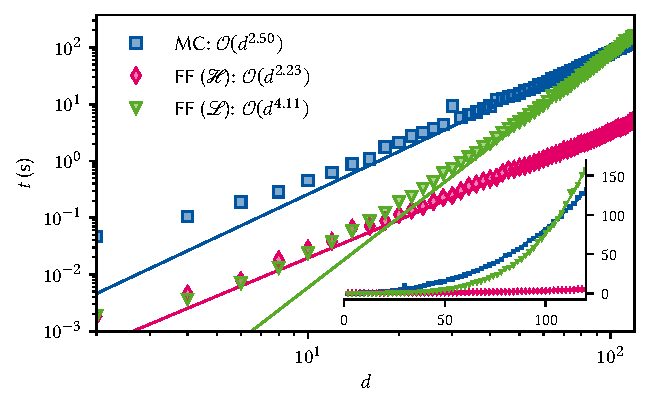
\includegraphics[width=\textwidth]{img/pdf/filter_functions/benchmark_MC_vs_FF}
    \caption[\imgsource{img/py/filter_functions/benchmark_monte_carlo.py}]{
        Performance of the formalism using \cref{eq:ff:control_matrix:pulse:freq:ff:calculation} compared to a Monte Carlo method for a single gate as a function of problem dimension $d$.
        Parameters are: $n_{\Delta t} = \num{1}, n_\alpha = 3, n_\mr{MC} = 100, f_\mr{UV} = 10^2/\Delta t, n_\omega = \num{500}$ where $n_\alpha$ is the number of noise operators considered, $n_\mr{MC}$ the number of Monte Carlo trajectories over which is averaged, and $n_\omega$ the number of frequency samples.
        The calculation using filter functions clearly outperforms \gls{mc} for small system sizes.
        For dimensions larger than $d\approx\num{100}$ (roughly equivalent to 7 qubits) Monte Carlo (blue squares) performs better than the \gls{ff} calculation with transfer matrices (green triangles) for this set of parameters and processor due to the better scaling behavior.
        Using conjugation by unitaries (orange diamonds) significantly outperforms \gls{mc} also for large dimensions.
        While the fits to $t = a d^b$ (lines) underestimate the leading order exponent due to the data not being in the asymptotic regime, they support the expected relationship of complexity between the approaches.
        The inset shows the same data on a linear scale, highlighting the different scaling behaviors for large $d$.
    }
    \label{fig:ff:performance:MC_vs_FF}
\end{figure*}

Quantifying the performance gain from using the control matrices' concatenation property to calculate fidelities of gate sequences is more difficult since it strongly depends on the number of gates occurring multiple times in the sequence (enabling reuse of precomputed control matrices) as well as the complexity of the individual gates.
The evaluation using the concatenation rule \cref{eq:ff:control_matrix:sequence:freq} performs asymptotically worse than the evaluation for a complete pulse according to \cref{eq:ff:control_matrix:pulse:freq:ff:calculation} because of higher powers of $d$ dominating the calculation in the former case.
Performing the $G$ matrix multiplications $\ctrlmat\gth{g}(\omega)\liouvQ\gth{g-1}$ from \cref{eq:ff:control_matrix:sequence:freq} is of order $\sim G n_\omega n_\alpha d^4$, with $G$ the number of pulses in the sequence.
Furthermore, calculating the transfer matrix of the total propagators $Q_{g-1}$ involves multiplication of $d\times d$ matrices for all $d^4$ combinations of basis elements amounting to $\sim G d^{b+4}$.
In case the Liouville representation of the individual pulses' total propagators $P_g$, $\liouvP\gth{g}$, have been precomputed, the latter computation can be made more efficient since one can just propagate the transfer matrices $\liouvP\gth{g}$ to obtain the cumulative transfer matrices for the sequence, $\liouvQ\gth{g}=\prod_{g^\prime=g}^0\liouvQ\gth{g^\prime}$, at cost $\sim G d^{2b}$.
The restriction to small dimensions does not apply for conjugation by unitaries as in this case the matrix multiplications involve $d\times d$ matrices and we do not have to compute the Liouville representation.
We thus obtain a more favorable asymptotic scaling of $\sim G n_\omega n_\alpha d^b$.

Utilizing the concatenation property in the Liouville representation thus corresponds to effectively reducing the number of times the calculations scaling with $\sim n_\omega n_\alpha d^4$ have to be carried out but incurs additional calculations scaling with $\sim d^{2b}$.
Accordingly, it provides a performance benefit if a sequence consists of either very complex pulses, in which case single repetitions already make the calculation much more efficient, or of few pulses that occur many times.
In the extremal case of $G$ repetitions of a single gate the benefit of employing the concatenation property is most pronounced and can be improved even further utilizing the simplifications laid out in \cref{sec:ff:performance:periodic_hamiltonians}.
Since matrix inversion has the same complexity as matrix multiplication and taking a matrix to the $G$ power requires $\order{\log G}$ matrix multiplications, \cref{eq:ff:control_matrix:sequence:periodic:simplified} should scale with $\sim n_\omega (n_\alpha d^4 + d^{2b} + d^{2b}\log{G})$ (the first two terms are due to the final matrix multiplications and are independent of $G$).
It hence allows for a vast speedup over \cref{eq:ff:control_matrix:sequence:freq} in that the asymptotic behavior as a function of the number of gates changes from $\sim G$ to $\sim\log G$.
An example of this is presented in \cref{sec:ff:examples:rabi_driving} for the context of Rabi driving.
Note that this closed form is a unique feature of the transfer matrix representation and not applicable to conjugation by unitaries.

